\subsection{Otras Relaciones}

\begin{table}[h]
	\subsubsection{Elementos}
	\begin{center}
		\begin{tabular}{| l | l | c |}
			\hline
			Concepto & Descripción & Representación \\ \hline
			
			Asociación 
			&
			\begin{tabular}[l]{@{}l@{}}
				Modela una relación no especificada, \\
				o una que no está representado por \\
				otro ArchiMate relación.
			\end{tabular}
			& 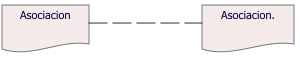
\includegraphics[width=0.4\linewidth]{imgs/relaciones/asociacion}
			\\\hline
			
			Especialización
			& 
			\begin{tabular}[l]{@{}l@{}}
				Indica que un elemento es un tipo \\
				particular de otro elemento.
			\end{tabular}
			& 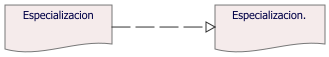
\includegraphics[width=0.4\linewidth]{imgs/relaciones/especializacion}
			\\\hline
			
			Unión
			& 
			\begin{tabular}[l]{@{}l@{}}
				Se usa para conectar relaciones \\
				del mismo tipo.
			\end{tabular}
			& 
\includegraphics[width=0.2\linewidth]{imgs/relaciones/union}
			\\\hline
			
		\end{tabular}
		\caption{Otras relaciones}
		\label{tab:otras}
	\end{center}
\end{table}